\begin{enumerate}[label=\thechapter.\arabic*,ref=\thechapter.\theenumi]
\item The value of the contour integral, $\oint_C \frac{z + 2}{z^2 + 2z + 2} \, dz$, where the contour $C$ is $\{ z : |z + 1 - \frac{3}{2}i| = 1 \}$, taken in the counter clockwise direction, is \\

\begin{enumerate}
  \item[(A)] $-\pi(1+j) $
  \item[(B)] $\pi(1+j)$
  \item[(C)] $\pi(1-j) $
  \item[(D)] $-\pi(1-j)$
\end{enumerate}

\hfill{(GATE EC 2023)}\\
\solution
\iffalse
\let\negmedspace\undefined
\let\negthickspace\undefined
\documentclass[journal,12pt,onecolumn]{IEEEtran}
\usepackage{cite}
\usepackage{amsmath,amssymb,amsfonts,amsthm}
\usepackage{algorithmic}
\usepackage{graphicx}
\usepackage{textcomp}
\usepackage{xcolor}
\usepackage{txfonts}
\usepackage{listings}
\usepackage{enumitem}
\usepackage{mathtools}
\usepackage{gensymb}
\usepackage{comment}
\usepackage[breaklinks=true]{hyperref}
\usepackage{tkz-euclide} % loads  TikZ and tkz-base
\usepackage{listings}
\usepackage[latin1]{inputenc}                                
\usepackage{color}                                            
\usepackage{array}                                            
\usepackage{longtable}                                       
\usepackage{calc}                                             
\usepackage{multirow}                                         
\usepackage{hhline}                                           
\usepackage{ifthen}                                           
\usepackage{lscape}
\usepackage{caption}
\usepackage{subcaption}


\newtheorem{theorem}{Theorem}[section]
\newtheorem{problem}{Problem}
\newtheorem{proposition}{Proposition}[section]
\newtheorem{lemma}{Lemma}[section]
\newtheorem{corollary}[theorem]{Corollary}
\newtheorem{example}{Example}[section]
\newtheorem{definition}[problem]{Definition}
%\newtheorem{thm}{Theorem}[section] 
%\newtheorem{defn}[thm]{Definition}
%\newtheorem{algorithm}{Algorithm}[section]
%\newtheorem{cor}{Corollary}
\newcommand{\BEQA}{\begin{eqnarray}}
\newcommand{\EEQA}{\end{eqnarray}}
\newcommand{\define}{\stackrel{\triangle}{=}}
\theoremstyle{remark}
\newtheorem{rem}{Remark}
%\bibliographystyle{ieeetr}

\begin{document}

%
\providecommand{\pr}[1]{\ensuremath{\Pr\left(#1\right)}}
\providecommand{\prt}[2]{\ensuremath{p_{#1}^{\left(#2\right)} }}        % own macro for this question
\providecommand{\qfunc}[1]{\ensuremath{Q\left(#1\right)}}
\providecommand{\sbrak}[1]{\ensuremath{{}\left[#1\right]}}
\providecommand{\lsbrak}[1]{\ensuremath{{}\left[#1\right.}}
\providecommand{\rsbrak}[1]{\ensuremath{{}\left.#1\right]}}
\providecommand{\brak}[1]{\ensuremath{\left(#1\right)}}
\providecommand{\lbrak}[1]{\ensuremath{\left(#1\right.}}
\providecommand{\rbrak}[1]{\ensuremath{\left.#1\right)}}
\providecommand{\cbrak}[1]{\ensuremath{\left\{#1\right\}}}
\providecommand{\lcbrak}[1]{\ensuremath{\left\{#1\right.}}
\providecommand{\rcbrak}[1]{\ensuremath{\left.#1\right\}}}
\newcommand{\sgn}{\mathop{\mathrm{sgn}}}
\providecommand{\abs}[1]{\left\vert#1\right\vert}
\providecommand{\res}[1]{\Res\displaylimits_{#1}} 
\providecommand{\norm}[1]{\left\lVert#1\right\rVert}
%\providecommand{\norm}[1]{\lVert#1\rVert}
\providecommand{\mtx}[1]{\mathbf{#1}}
\providecommand{\mean}[1]{E\left[ #1 \right]}
\providecommand{\cond}[2]{#1\middle|#2}
\providecommand{\fourier}{\overset{\mathcal{F}}{ \rightleftharpoons}}
\newenvironment{amatrix}[1]{%
  \left(\begin{array}{@{}*{#1}{c}|c@{}}
}{%
  \end{array}\right)
}
%\providecommand{\hilbert}{\overset{\mathcal{H}}{ \rightleftharpoons}}
%\providecommand{\system}{\overset{\mathcal{H}}{ \longleftrightarrow}}
        %\newcommand{\solution}[2]{\textbf{Solution:}{#1}}
\newcommand{\solution}{\noindent \textbf{Solution: }}
\newcommand{\cosec}{\,\text{cosec}\,}
\providecommand{\dec}[2]{\ensuremath{\overset{#1}{\underset{#2}{\gtrless}}}}
\newcommand{\myvec}[1]{\ensuremath{\begin{pmatrix}#1\end{pmatrix}}}
\newcommand{\mydet}[1]{\ensuremath{\begin{vmatrix}#1\end{vmatrix}}}
\newcommand{\myaugvec}[2]{\ensuremath{\begin{amatrix}{#1}#2\end{amatrix}}}
\providecommand{\rank}{\text{rank}}
\providecommand{\pr}[1]{\ensuremath{\Pr\left(#1\right)}}
\providecommand{\qfunc}[1]{\ensuremath{Q\left(#1\right)}}
        \newcommand*{\permcomb}[4][0mu]{{{}^{#3}\mkern#1#2_{#4}}}
\newcommand*{\perm}[1][-3mu]{\permcomb[#1]{P}}
\newcommand*{\comb}[1][-1mu]{\permcomb[#1]{C}}
\providecommand{\qfunc}[1]{\ensuremath{Q\left(#1\right)}}
\providecommand{\gauss}[2]{\mathcal{N}\ensuremath{\left(#1,#2\right)}}
\providecommand{\diff}[2]{\ensuremath{\frac{d{#1}}{d{#2}}}}
\providecommand{\myceil}[1]{\left \lceil #1 \right \rceil }
\newcommand\figref{Fig.~\ref}
\newcommand\tabref{Table~\ref}
\newcommand{\sinc}{\,\text{sinc}\,}
\newcommand{\rect}{\,\text{rect}\,}
%%
%       %\newcommand{\solution}[2]{\textbf{Solution:}{#1}}
%\newcommand{\solution}{\noindent \textbf{Solution: }}
%\newcommand{\cosec}{\,\text{cosec}\,}
%\numberwithin{equation}{section}
%\numberwithin{equation}{subsection}
%\numberwithin{problem}{section}
%\numberwithin{definition}{section}
%\makeatletter
%\@addtoreset{figure}{problem}
%\makeatother

%\let\StandardTheFigure\thefigure
\let\vec\mathbf

\bibliographystyle{IEEEtran}

\renewcommand{\thefigure}{\theenumi}
\renewcommand{\thetable}{\theenumi}
%\renewcommand{\theequation}{\theenumi}
Q:Which one of the options given is the inverse Laplace transform of $\frac{1}{s^3-s}$?\\
$u(t)$ denotes the unit-step function.
\begin{enumerate}[label=(\Alph*)]
\item $\left(-1+\frac{1}{2}e^-t+\frac{1}{2}e^t\right)u(t)$\\
\item $\left(\frac{1}{3}e^-t-e^t\right)u(t)$\\
\item $\left(-1+\frac{1}{2}e^{-(t-1)}+\frac{1}{2}e^{(t-1)}\right)u(t-1)$\\
\item $\left(-1-\frac{1}{2}e^{-(t-1)}-\frac{1}{2}e^{(t-1)}\right)u(t-1)$\\
\end{enumerate}
\hfill(GATE ME 2023)

%\end{document}

\pagebreak

\item The function $f(Z)=\frac{1}{Z-1}$ of a complex variable Z is integrated on a closed contour in an anti-clockwise direction. For which of the following contours, does this integral have a non-zero value?\\
\brak{A}$\abs{z-2}=0.01$\\
\brak{B}$\abs{z-1}=0.1$\\
\brak{C}$\abs{z-3}=5$\\
\brak{D}$\abs{z}=2$\\
\hfill(GATE 2023 BM)\\
\solution
\iffalse
\let\negmedspace\undefined
\let\negthickspace\undefined
\documentclass[journal,12pt,twocolumn]{IEEEtran}
\usepackage{cite}
\usepackage{amsmath,amssymb,amsfonts,amsthm}
\usepackage{algorithmic}
\usepackage{graphicx}
\usepackage{textcomp}
\usepackage{xcolor}
\usepackage{txfonts}
\usepackage{listings}
\usepackage{enumitem}
\usepackage{mathtools}
\usepackage{gensymb}
\usepackage{comment}
\usepackage[breaklinks=true]{hyperref}
\usepackage{tkz-euclide} 
\usepackage{listings}
\usepackage{gvv}                                        
\def\inputGnumericTable{}                                 
\usepackage[latin1]{inputenc}                                
\usepackage{color}                                            
\usepackage{array}                                            
\usepackage{longtable}                              
\usepackage{calc}                                             
\usepackage{multirow}                                         
\usepackage{hhline}                                           
\usepackage{ifthen}                                           
\usepackage{lscape}

\newtheorem{theorem}{Theorem}[section]
\newtheorem{problem}{Problem}
\newtheorem{proposition}{Proposition}[section]
\newtheorem{lemma}{Lemma}[section]
\newtheorem{corollary}[theorem]{Corollary}
\newtheorem{example}{Example}[section]
\newtheorem{definition}[problem]{Definition}
\newcommand{\BEQA}{\begin{eqnarray}}
\newcommand{\EEQA}{\end{eqnarray}}
\newcommand{\define}{\stackrel{\triangle}{=}}
\theoremstyle{remark}
\newtheorem{rem}{Remark}
\begin{document}

\bibliographystyle{IEEEtran}
\vspace{3cm}

\title{GATE 2023 BM}
\author{EE23BTECH11020 - Raghava Ganji$^{*}$% <-this % stops a space
}
\maketitle
\newpage
\bigskip

\renewcommand{\thefigure}{\theenumi}
\renewcommand{\thetable}{\theenumi}

\textbf{GATE 2023 BM.48:}
The function $f(z)=\frac{1}{z-1}$ of a complex variable z on a closed contour in an anti-clockwise direction.For which of the following contours, does this integral have a non-zero value?\\
\brak{A}$\abs{z-2}=0.01$\\
\brak{B}$\abs{z-1}=0.1$\\
\brak{C}$\abs{z-3}=5$\\
\brak{D}$\abs{z}=2$\\
\solution\\
\fi
Cauchy's Integral Formula and Residue Theorem.
\begin{align}
\oint_{c}f\brak z&=2\pi jRes\sbrak{f\brak z,z_0}\label{eq:CIF}\\
Res\sbrak{f\brak z,z_0}&=\lim_{z\to z_0}\sbrak{\brak{z-z_0}f\brak z}\label{eq:Res Thm}
\end{align}
Here $z_0$ is pole of the f\brak z\\
Using \eqref{eq:CIF}
\begin{align}
\oint_{c}\frac{1}{z-1}dz &=2\pi jRes\sbrak{\frac{1}{z-1},1}
\end{align}
\begin{enumerate}
\item For option A the pole is outside the contour, then Residue is zero.\\
\begin{figure}[h!]
    \centering
    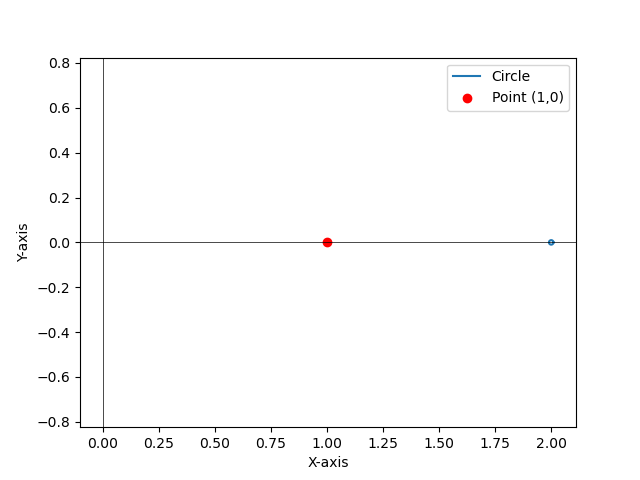
\includegraphics[width=1\columnwidth]{2023/BM/48/figs/plotg231.png}
    \caption{graph of option A}
\end{figure}
\begin{align}
\implies\oint_{c}\frac{1}{z-1}dz &=2\pi j\brak{0}\\
\implies 0
\end{align}
\item For option B the pole is inside the contour.\\
\begin{figure}[h!]
    \centering
    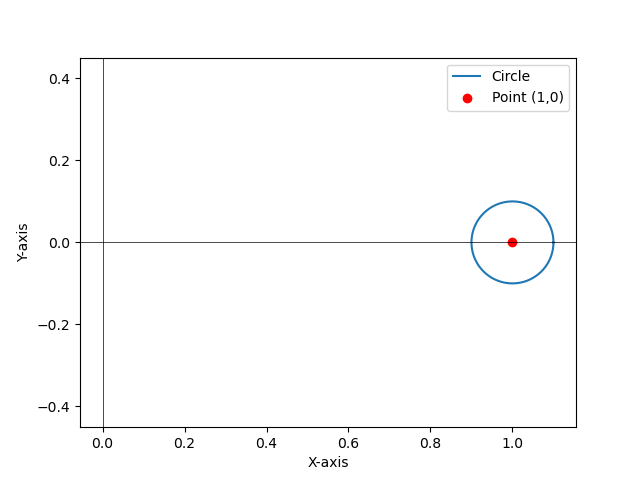
\includegraphics[width=1\columnwidth]{2023/BM/48/figs/plotg232.png}
    \caption{graph of option B}
\end{figure}
Then, using \eqref{eq:Res Thm}
\begin{align}
Res\sbrak{\frac{1}{z-1},1} &=\lim_{z\to 1}\brak{z-1}\frac{1}{z-1}\\
&=1\\
\implies \oint_{c}\frac{1}{z-1}dz&=2\pi j\brak 1\\
\implies 2\pi j
\end{align}
\item For option C the pole is inside the contour.\\
\begin{figure}[h!]
    \centering
    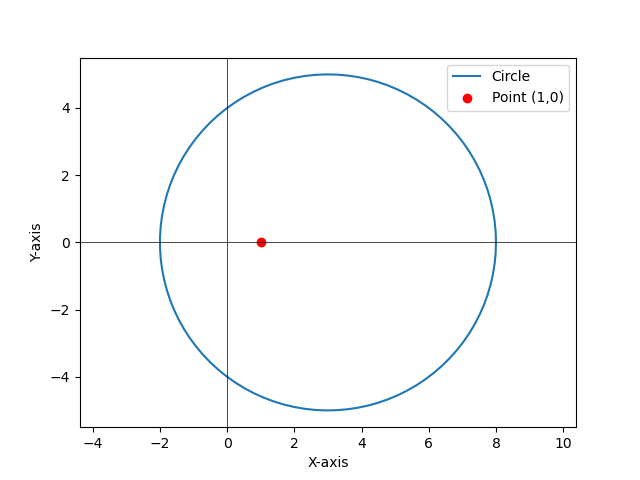
\includegraphics[width=1\columnwidth]{2023/BM/48/figs/plotg233.png}
    \caption{graph of option C}
\end{figure}
Then, using \eqref{eq:Res Thm}
\begin{align}
Res\sbrak{\frac{1}{z-1},1} &=\lim_{z\to 1}\brak{z-1}\frac{1}{z-1}\\
&=1\\
\implies \oint_{c}\frac{1}{z-1}dz&=2\pi j\brak 1\\
\implies 2\pi j
\end{align}
\item For option D the pole is inside the contour.\\
\begin{figure}[h!]
    \centering
    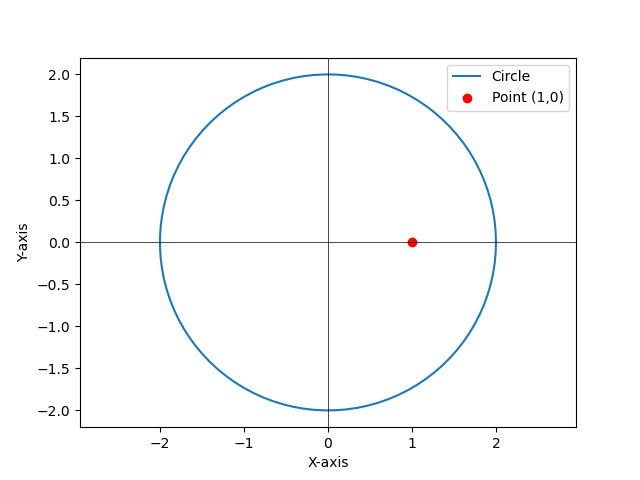
\includegraphics[width=1\columnwidth]{2023/BM/48/figs/plotg234.png}
    \caption{graph of option D}
\end{figure}
Then, using \eqref{eq:Res Thm}
\begin{align}
Res\sbrak{\frac{1}{z-1},1} &=\lim_{z\to 1}\brak{z-1}\frac{1}{z-1}\\
&=1\\
\implies \oint_{c}\frac{1}{z-1}dz&=2\pi j\brak 1\\
\implies 2\pi j
\end{align}
\end{enumerate}
We can conclude that for options B,C,D contours have the non-zero value for this integral.
%\end{document}

\newpage
\item Consider the contour integral $\oint \frac{dz}{z^4 + z^3 - 2z^2}$, along the curve $|z| = 3$ oriented in the counterclockwise direction. If $\text{Res}[f, z_0]$ denotes the residue of $f(z)$ at the point $z_0$, then which of the following are TRUE? \\
\begin{itemize}
    \item (A) $\text{Res}[f, 0] = -\frac{1}{4}$
    \item (B) $\text{Res}[f, 1] = \frac{1}{3}$
    \item (C) $\text{Res}[f, -2] = -\frac{1}{12}$
    \item (D) $\text{Res}[f, 2] = -1$
\end{itemize}
\hfill{(GATE NM 2023)}\\
\solution
\newpage
\end{enumerate}
